\documentclass[tikz, border=4pt]{standalone}
\usepackage{tikz}
\usepackage{pgfplots}
\pgfplotsset{compat=1.18}
\begin{document}
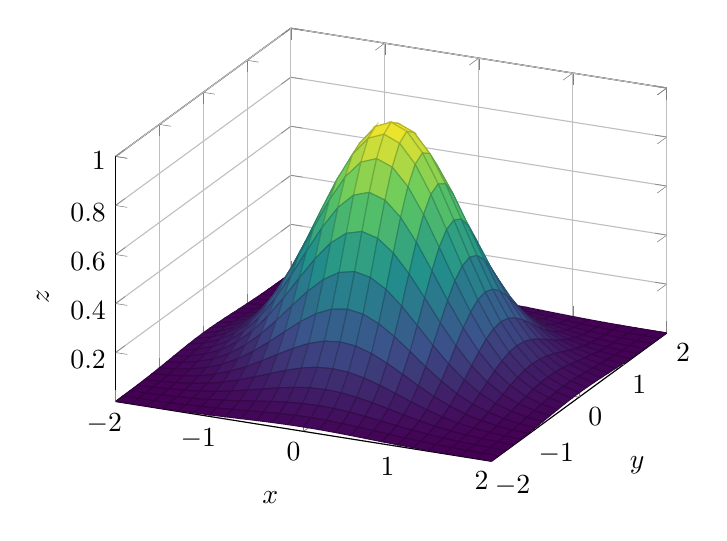
\begin{tikzpicture}[x=1cm, y=1cm]
  \definecolor{tdc1}{HTML}{1E5BD6}

  \begin{axis}[
    at={(0cm,-5.5cm)},
    anchor=south west,
    scale only axis,
    width=7cm,
    height=5.5cm,
    xmin=-2,
    xmax=2,
    ymin=-2,
    ymax=2,
    zmin=0.0003,
    zmax=1,
    view={25}{30},
    xtick={-2,-1,0,1,2},
    ytick={-2,-1,0,1,2},
    ztick={0.2,0.4,0.6,0.8,1},
    grid=major,
    xlabel={$x$},
    ylabel={$y$},
    zlabel={$z$},
    colormap={tdmap}{rgb255(0cm)=(68,1,84); rgb255(1cm)=(59,82,139); rgb255(2cm)=(33,145,140); rgb255(3cm)=(94,201,98); rgb255(4cm)=(253,231,37)},
    point meta min=0.0003,
    point meta max=1
  ]
    \addplot3[surf, shader=faceted, domain=-2:2, y domain=-2:2, samples=25, forget plot] {exp((-((x)^(2)+(y)^(2))))};
  \end{axis}
\end{tikzpicture}
\end{document}
